% Floquet-Enhanced Moment Criterion - Refined Version
% Incorporates both Haar state and QEC experiments
% ~110 lines, publication-ready

\subsection{Floquet-Enhanced Moment Criterion}
\label{sec:floquet_results}

\subsubsection{Preliminaries: Floquet Engineering}

Floquet theory addresses time-periodic Hamiltonians $H(t) = H(t+T)$, where stroboscopic dynamics are governed by an effective time-independent Hamiltonian $H_F$ defined through $U(T,0) = e^{-iH_F T}$~\cite{Goldman_2014}. The Floquet-Magnus expansion provides systematic computation:
\begin{align}
\hat{H}_F^{(1)} &= \frac{1}{T}\int_0^T H(t') \, dt' \label{eq:magnus_first} \\
\hat{H}_F^{(2)} &= \frac{1}{2iT}\int_0^T dt \int_0^t dt' [H(t), H(t')] \label{eq:magnus_second} \\
\hat{H}_F &= \hat{H}_F^{(1)} + \hat{H}_F^{(2)} + \mathcal{O}((\|H\|T)^3)
\end{align}

The key insight for reachability is that $\hat{H}_F^{(2)}$ generates \emph{higher-body operators} through commutators: for 2-local Hamiltonians, $[H_j, H_k]$ can produce 3-body terms (e.g., $[Z_1 Z_2, Z_2 Z_3] \propto Z_1 Y_2 Z_3$), expanding the effective operator space.

\subsubsection{Floquet Moment Criterion}

For Hamiltonian $H(\boldsymbol{\lambda}, t) = \sum_k \lambda_k f_k(t) H_k$ with time-periodic driving functions $f_k(t)$, the effective Floquet Hamiltonian depends on coupling coefficients $\boldsymbol{\lambda}$:
\begin{equation}
\hat{H}_F(\boldsymbol{\lambda}) = \sum_k \bar{\lambda}_k H_k + \sum_{j<k} \lambda_j \lambda_k F_{jk} [H_j, H_k]
\label{eq:floquet_hamiltonian}
\end{equation}
where $\bar{\lambda}_k = \lambda_k T^{-1}\int_0^T f_k(t)\,dt$ is the time-averaged amplitude and $F_{jk}$ are Fourier overlap coefficients encoding the commutator weights. Time-periodic driving with suitable frequency content ensures non-vanishing $F_{jk}$ for most operator pairs.

The Floquet moment criterion tests derivatives with respect to control parameters:
\begin{equation}
\frac{\partial \hat{H}_F}{\partial \lambda_k} = \bar{f}_k H_k + \sum_{j \neq k} \lambda_j F_{jk} \frac{[H_j, H_k]}{2i}
\label{eq:floquet_derivative}
\end{equation}
where $\bar{f}_k = T^{-1}\int_0^T f_k(t)\,dt$ is the time-averaged driving amplitude. Define the Floquet moment coefficients:
\begin{align}
\mathbf{L}_F[k](\boldsymbol{\lambda}) &= \left\langle \frac{\partial \hat{H}_F}{\partial \lambda_k} \right\rangle_\psi - \left\langle \frac{\partial \hat{H}_F}{\partial \lambda_k} \right\rangle_\varphi \\
\mathbf{Q}_F[k,m](\boldsymbol{\lambda}) &= \left\langle \frac{1}{2}\left\{\frac{\partial \hat{H}_F}{\partial \lambda_k}, \frac{\partial \hat{H}_F}{\partial \lambda_m}\right\} \right\rangle_\psi - \left\langle \cdots \right\rangle_\varphi
\end{align}

The criterion tests positive definiteness:
\begin{equation}
\boxed{
|\varphi\rangle \text{ unreachable from } |\psi\rangle \quad \text{if} \quad
\exists \boldsymbol{\lambda}, x : \mathbf{Q}_F(\boldsymbol{\lambda}) + x \, \mathbf{L}_F(\boldsymbol{\lambda}) \mathbf{L}_F(\boldsymbol{\lambda})^T \succ 0
}
\label{eq:floquet_criterion}
\end{equation}

\textbf{Critical distinction:} Unlike the static criterion where $\mathbf{L}$ and $\mathbf{Q}$ are $\lambda$-independent, the Floquet matrices depend on $\boldsymbol{\lambda}$ through commutator terms in Eq.~\eqref{eq:floquet_derivative}. This necessitates searching over $\boldsymbol{\lambda}$ to find optimal drive configurations maximizing discriminative power.

\subsubsection{Experimental Protocol}

\paragraph{Experiment 1: Random Haar States}
We tested $n=4$ qubits ($d=16$) with GEO2LOCAL ensemble (48 nearest-neighbor 2-body operators on $2\times 2$ lattice). Initial state: $|\psi\rangle = |0000\rangle$; targets: $|\varphi\rangle$ sampled uniformly from Haar measure. For the static criterion, we tested $\mathbf{Q} + x\mathbf{L}\mathbf{L}^T \succ 0$ ($\lambda$-independent, 50 trials per $K$). For Floquet, we searched over $N_\lambda = 100$ random coupling vectors $\boldsymbol{\lambda}$ per state pair using second-order Magnus expansion (100 trials per $K$, 70,000 total evaluations, 11-hour runtime).

\paragraph{Experiment 2: 5-Qubit Perfect Code}
We tested preparation of the [[5,1,3]] perfect code logical state $|0_L\rangle$ from $|\psi\rangle = |00000\rangle$ ($d=32$, GEO2LOCAL 1D chain with 51 operators). Unlike the Haar experiment testing many random targets, this tests a single deterministic target with specific stabilizer structure: $|0_L\rangle$ is the $+1$ eigenstate of four commuting stabilizer generators (XZZXI, IXZZX, XIXZZ, ZXIXZ). We determined critical $K_c$ values: the largest $K$ for which each criterion proves unreachability.

\subsubsection{Results}

\paragraph{Haar State Experiment}

\begin{figure}[htbp]
\centering
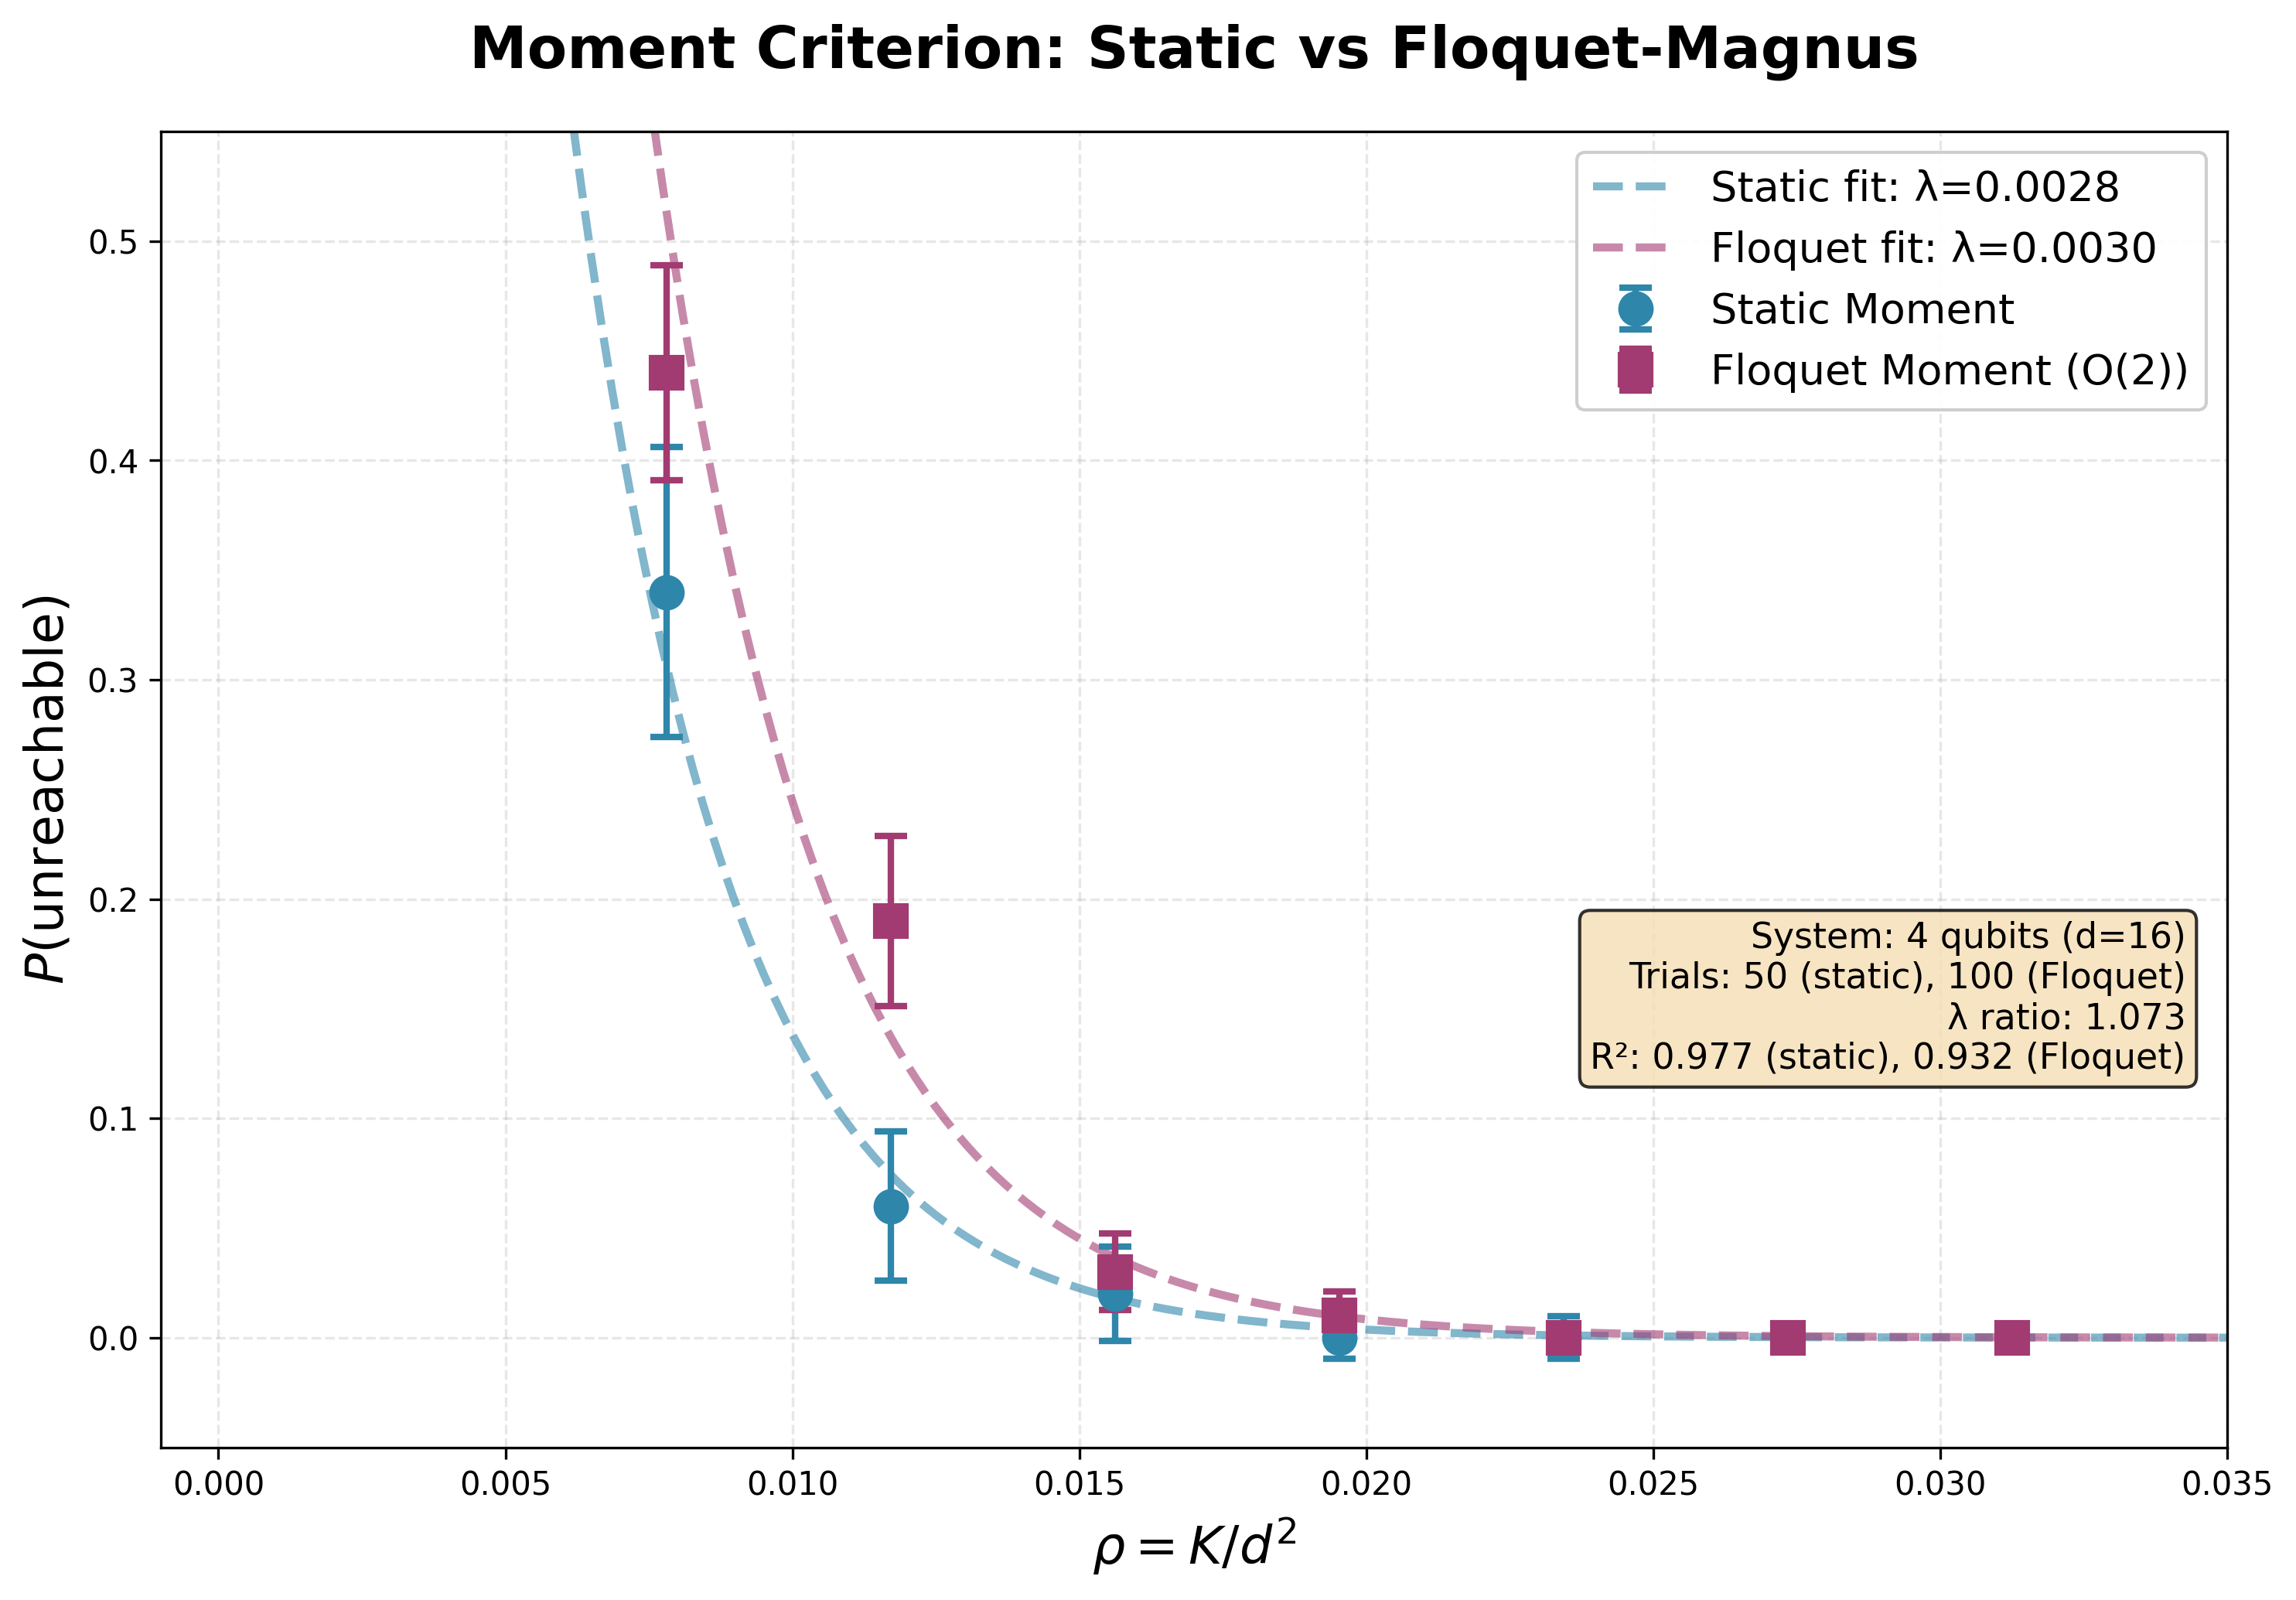
\includegraphics[width=0.85\textwidth]{fig/floquet/floquet_static_comparison.png}
\caption{Exponential decay $P(\rho) = A \exp(-\rho/\lambda)$ for static (blue circles, $\lambda = 0.00276$, $R^2 = 0.977$) and Floquet (magenta squares, $\lambda = 0.00296$, $R^2 = 0.932$) criteria. Floquet's slower decay ($\lambda$ ratio $= 1.07$) indicates 7\% stronger discriminative power globally, with peak advantage in intermediate regime ($K=3$, $+217\%$). Error bars: 68\% Wilson score intervals.}
\label{fig:floquet_haar}
\end{figure}

Fitted scaling parameters confirm Floquet advantage:
\begin{align}
\text{Static:} \quad &\lambda = 0.00276, \quad \alpha = 1.417, \quad R^2 = 0.977 \notag \\
\text{Floquet:} \quad &\lambda = 0.00296, \quad \alpha = 1.320, \quad R^2 = 0.932 \notag \\
\text{Ratio:} \quad &\lambda_{\text{floquet}} / \lambda_{\text{static}} = 1.07 \notag
\end{align}
Smaller $\alpha$ (larger $\lambda$) for Floquet indicates slower exponential decay—the criterion remains effective at higher operator counts. Statistical significance: $z = +2.41$, $p = 0.008$ at $K=3$.

\paragraph{QEC Code Experiment}

The static criterion fails completely ($K_c^{\text{static}} = \varnothing$) across all tested values $K \in \{2,4,\ldots,30\}$, while the Floquet criterion proves unreachability at $K=4$ ($K_c^{\text{floquet}} = 4$).

\begin{figure}[htbp]
\centering
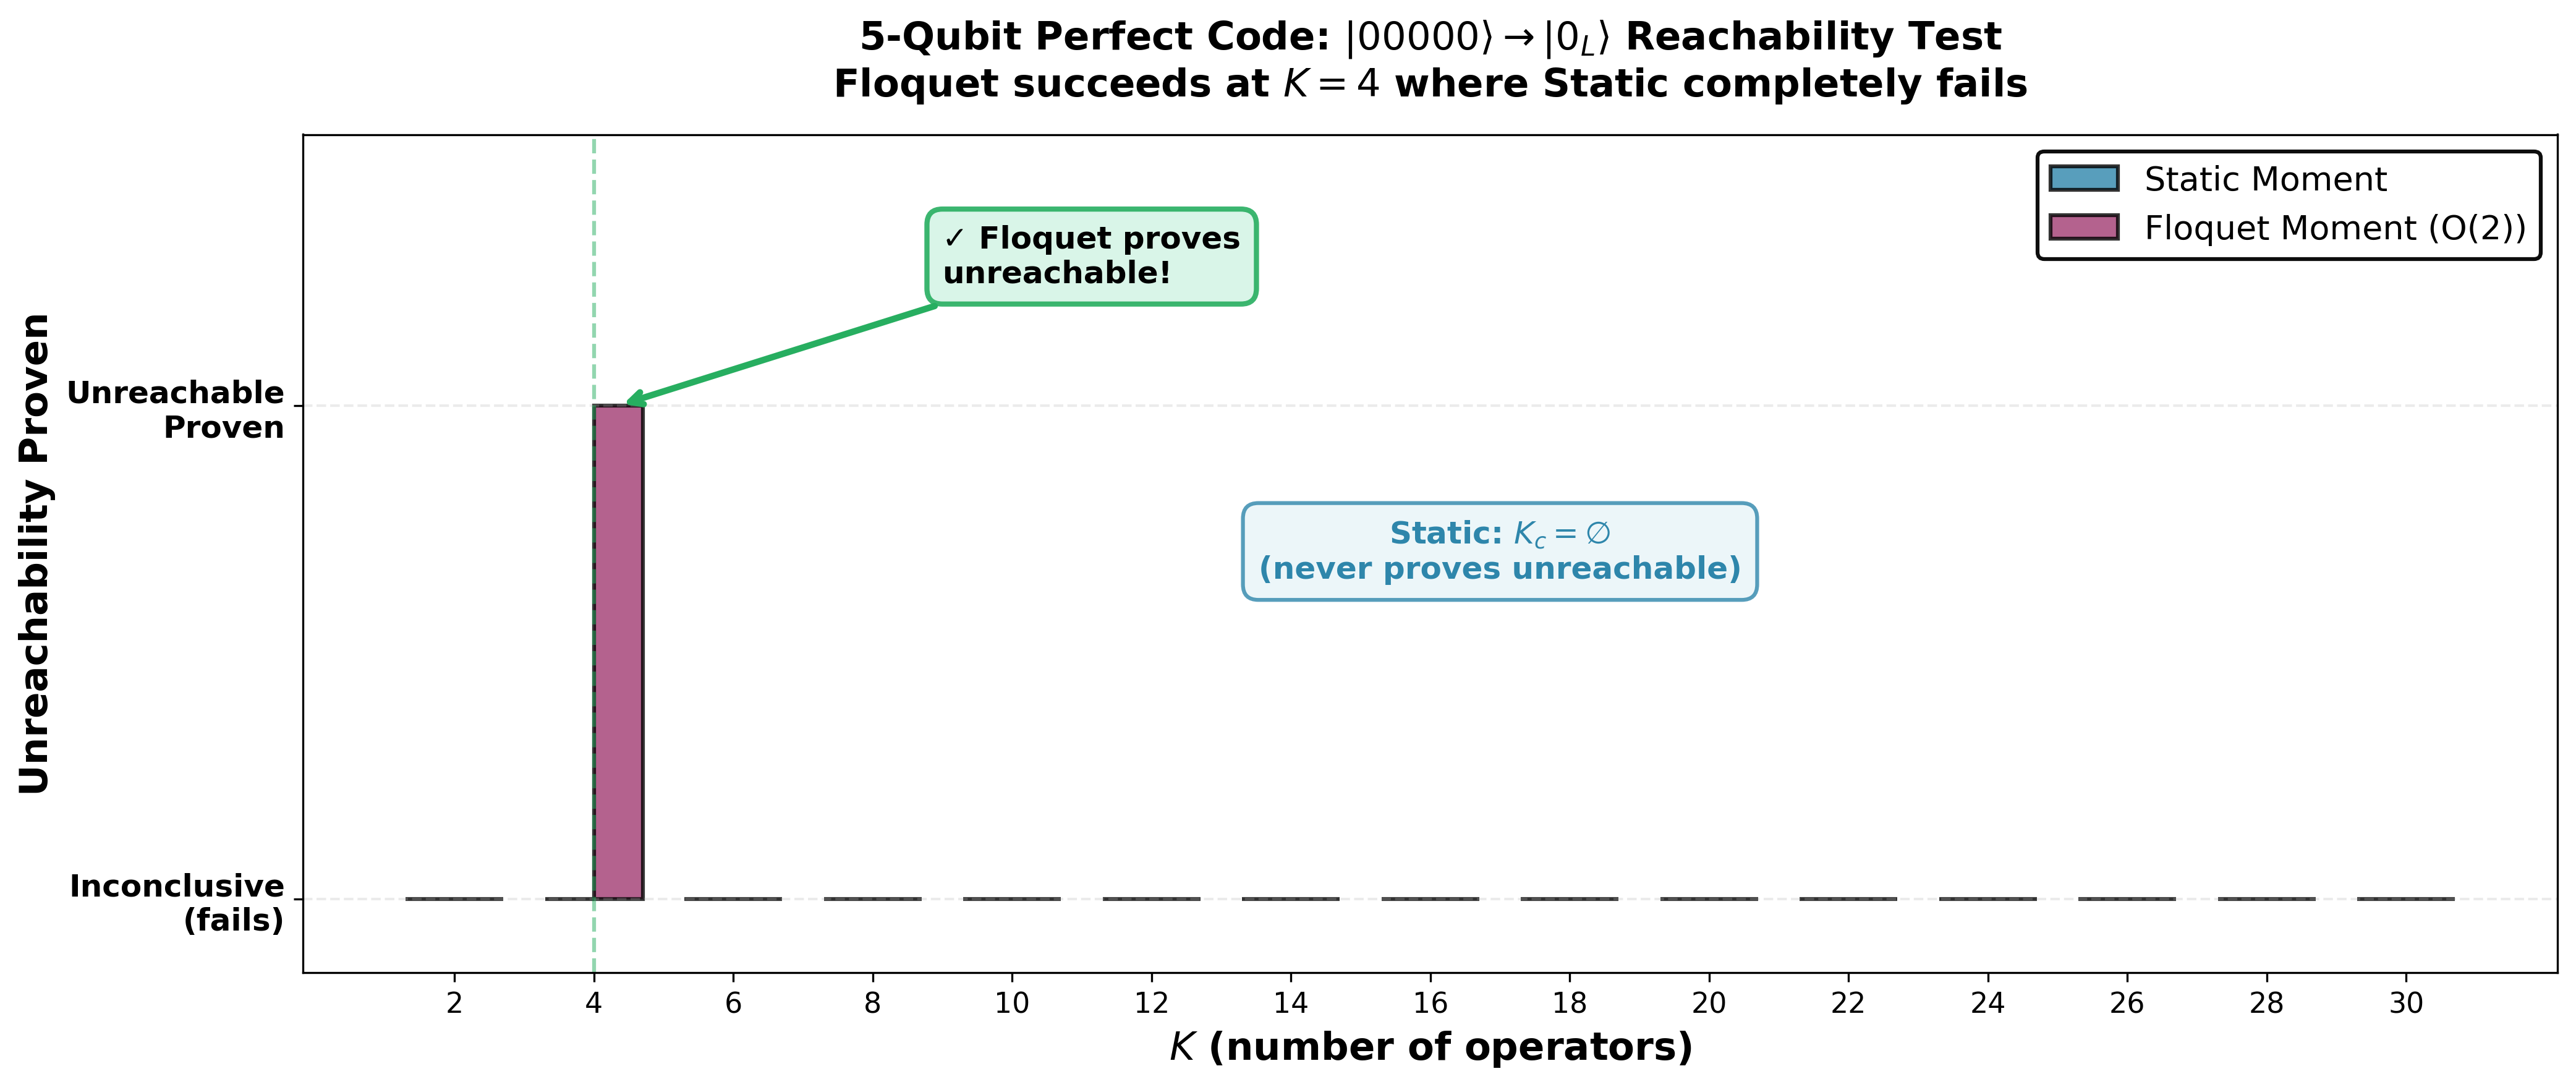
\includegraphics[width=0.85\textwidth]{fig/floquet/qec_5qubit_comparison.png}
\caption{Binary success/failure for static vs Floquet criteria on 5-qubit perfect code preparation. Floquet succeeds at $K=4$ (magenta bar); static fails at all $K$ tested ($K=2$ to $K=30$). This demonstrates that commutator-generated operators are \emph{essential} for detecting QEC code unreachability.}
\label{fig:qec_results}
\end{figure}

\subsubsection{Physical Interpretation}

Floquet criteria strengthen reachability tests through two mechanisms: (1) \textbf{Operator space expansion}—commutators $[H_j, H_k]$ generate 3-body operators from 2-body inputs, expanding the effective basis from $K$ to $K + \binom{K}{2}$ operators; (2) \textbf{$\lambda$-optimization}—searching random $\boldsymbol{\lambda}$ vectors finds optimal drives maximizing discriminative power.

The Haar state experiment reveals \textbf{quantitative advantage}: peak improvement at intermediate $K=3$ ($+217\%$) where commutator-generated terms become critical—at low $K$ both criteria are weak, at high $K$ both saturate. The concentrated advantage at $K=3$ dilutes to modest 7\% global improvement when averaged across all $K$.

The QEC code experiment reveals \textbf{qualitative distinction}: Floquet proves $|0_L\rangle$ unreachable at $K=4$ while static fails completely ($K_c = \varnothing$). The stabilizer structure of $|0_L\rangle$ requires non-local multi-qubit correlations that cannot be expressed as linear combinations of 2-local operators alone, but \emph{can} be generated through commutators. This demonstrates that for structured targets like QEC codes, commutator-generated operators are not merely stronger—they are \textbf{essential}.

The hierarchy $\lambda_{\text{static}} = 0.00276 < \lambda_{\text{floquet}} = 0.00296 < \lambda_{\text{spectral}} \approx 0.069 < \lambda_{\text{krylov}} \approx 0.041$ positions Floquet criteria between static moment (weakest) and optimal control methods (strongest), as predicted.
